\begin{exercise}
      {ID-a73d8600ba60329bc9f19f3d89589618a1cb2e30}
      {Oberflächentemperatur}
  \ifproblem\problem\par
    % <PROBLEM>
    An einem Tag im Frühherbst wird die
    Oberflächentemperatur eines Sees gemessen.
    Der Temperaturverlauf kann annähernd durch
    die Funktion $O$ mit
    \begin{equation*}
    O(t)=-\frac{1}{300}t^3+\num{0.12}t^2-\num{1.08}t+\num{19}
    \qquad
    0\leq t\leq24\text{ in h, $O(t)$ in ${}^\circ C$}
    \end{equation*}
    modelliert werden. Die folgende Abbildung zeigt den zugehörigen
    Graphen:
    \begin{center}
    %<OCTAVE>
    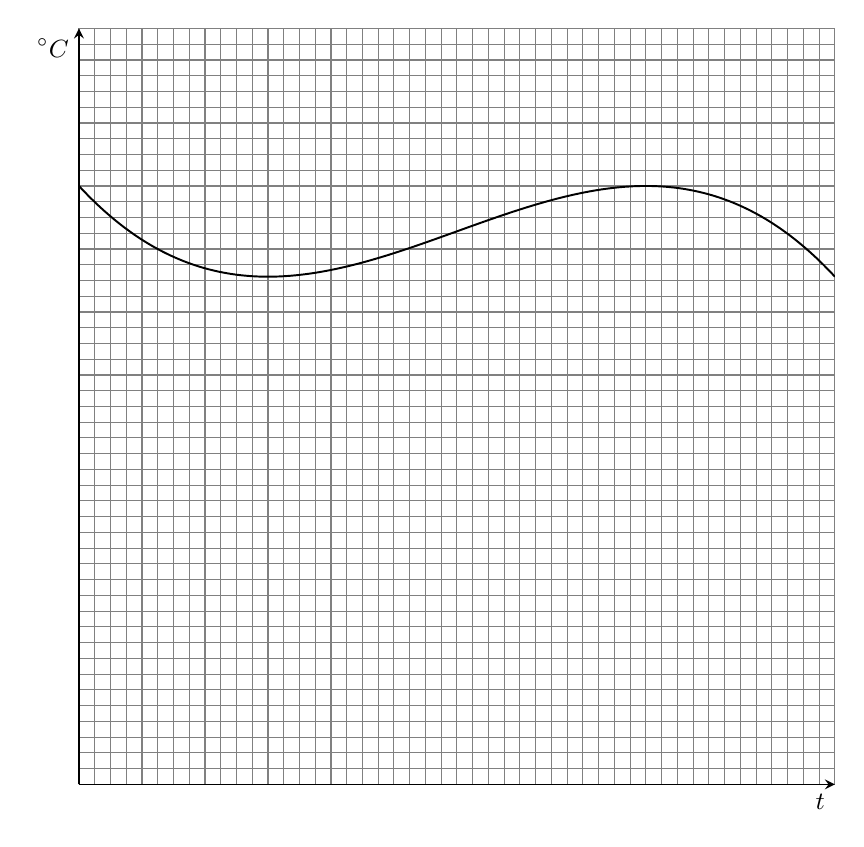
\begin{tikzpicture}[scale=0.400]
      % grid
      \draw[draw=black!50!white] (0.000, 0.000) grid[step=0.5] (24.000, 24.000);
      % x-axis
      \draw[line width=0.6pt, ->, >=stealth] (0.000, 0) -- (24.000, 0) node[below left] {\small$t$};
      % y-axis
      \draw[line width=0.6pt, ->, >=stealth] (0, 0.000) -- (0, 24.000) node[below left] {\small${}^\circ C$};
      % function: f(x)=-\num{0.0033333}x^{3}+\num{0.12}x^{2}-\num{1.08}x+\num{19}
      \begin{scope}[line width=0.7pt]
        \clip (0.000, 0.000) rectangle (24.000, 24.000);
        \draw plot[smooth] coordinates
        {
          (  0.000,  19.000) (  0.100,  18.893) (  0.200,  18.789)
          (  0.300,  18.687) (  0.400,  18.587) (  0.500,  18.490)
          (  0.600,  18.394) (  0.700,  18.302) (  0.800,  18.211)
          (  0.900,  18.123) (  1.000,  18.037) (  1.100,  17.953)
          (  1.200,  17.871) (  1.300,  17.791) (  1.400,  17.714)
          (  1.500,  17.639) (  1.600,  17.566) (  1.700,  17.494)
          (  1.800,  17.425) (  1.900,  17.358) (  2.000,  17.293)
          (  2.100,  17.230) (  2.200,  17.169) (  2.300,  17.110)
          (  2.400,  17.053) (  2.500,  16.998) (  2.600,  16.945)
          (  2.700,  16.893) (  2.800,  16.844) (  2.900,  16.796)
          (  3.000,  16.750) (  3.100,  16.706) (  3.200,  16.664)
          (  3.300,  16.623) (  3.400,  16.584) (  3.500,  16.547)
          (  3.600,  16.512) (  3.700,  16.478) (  3.800,  16.446)
          (  3.900,  16.415) (  4.000,  16.387) (  4.100,  16.359)
          (  4.200,  16.334) (  4.300,  16.310) (  4.400,  16.287)
          (  4.500,  16.266) (  4.600,  16.247) (  4.700,  16.229)
          (  4.800,  16.212) (  4.900,  16.197) (  5.000,  16.183)
          (  5.100,  16.171) (  5.200,  16.160) (  5.300,  16.151)
          (  5.400,  16.142) (  5.500,  16.135) (  5.600,  16.130)
          (  5.700,  16.125) (  5.800,  16.122) (  5.900,  16.121)
          (  6.000,  16.120) (  6.100,  16.121) (  6.200,  16.122)
          (  6.300,  16.125) (  6.400,  16.129) (  6.500,  16.135)
          (  6.600,  16.141) (  6.700,  16.148) (  6.800,  16.157)
          (  6.900,  16.166) (  7.000,  16.177) (  7.100,  16.188)
          (  7.200,  16.201) (  7.300,  16.214) (  7.400,  16.228)
          (  7.500,  16.244) (  7.600,  16.260) (  7.700,  16.277)
          (  7.800,  16.295) (  7.900,  16.314) (  8.000,  16.333)
          (  8.100,  16.354) (  8.200,  16.375) (  8.300,  16.397)
          (  8.400,  16.420) (  8.500,  16.443) (  8.600,  16.467)
          (  8.700,  16.492) (  8.800,  16.517) (  8.900,  16.543)
          (  9.000,  16.570) (  9.100,  16.597) (  9.200,  16.625)
          (  9.300,  16.654) (  9.400,  16.683) (  9.500,  16.712)
          (  9.600,  16.742) (  9.700,  16.773) (  9.800,  16.803)
          (  9.900,  16.835) ( 10.000,  16.867) ( 10.100,  16.899)
          ( 10.200,  16.931) ( 10.300,  16.964) ( 10.400,  16.998)
          ( 10.500,  17.031) ( 10.600,  17.065) ( 10.700,  17.099)
          ( 10.800,  17.134) ( 10.900,  17.168) ( 11.000,  17.203)
          ( 11.100,  17.238) ( 11.200,  17.274) ( 11.300,  17.309)
          ( 11.400,  17.345) ( 11.500,  17.380) ( 11.600,  17.416)
          ( 11.700,  17.452) ( 11.800,  17.488) ( 11.900,  17.524)
          ( 12.000,  17.560) ( 12.100,  17.596) ( 12.200,  17.632)
          ( 12.300,  17.668) ( 12.400,  17.704) ( 12.500,  17.740)
          ( 12.600,  17.775) ( 12.700,  17.811) ( 12.800,  17.846)
          ( 12.900,  17.882) ( 13.000,  17.917) ( 13.100,  17.952)
          ( 13.200,  17.986) ( 13.300,  18.021) ( 13.400,  18.055)
          ( 13.500,  18.089) ( 13.600,  18.122) ( 13.700,  18.156)
          ( 13.800,  18.189) ( 13.900,  18.221) ( 14.000,  18.253)
          ( 14.100,  18.285) ( 14.200,  18.317) ( 14.300,  18.347)
          ( 14.400,  18.378) ( 14.500,  18.408) ( 14.600,  18.437)
          ( 14.700,  18.466) ( 14.800,  18.495) ( 14.900,  18.523)
          ( 15.000,  18.550) ( 15.100,  18.577) ( 15.200,  18.603)
          ( 15.300,  18.628) ( 15.400,  18.653) ( 15.500,  18.677)
          ( 15.600,  18.700) ( 15.700,  18.723) ( 15.800,  18.745)
          ( 15.900,  18.766) ( 16.000,  18.787) ( 16.100,  18.806)
          ( 16.200,  18.825) ( 16.300,  18.843) ( 16.400,  18.860)
          ( 16.500,  18.876) ( 16.600,  18.892) ( 16.700,  18.906)
          ( 16.800,  18.919) ( 16.900,  18.932) ( 17.000,  18.943)
          ( 17.100,  18.954) ( 17.200,  18.963) ( 17.300,  18.972)
          ( 17.400,  18.979) ( 17.500,  18.985) ( 17.600,  18.991)
          ( 17.700,  18.995) ( 17.800,  18.998) ( 17.900,  18.999)
          ( 18.000,  19.000) ( 18.100,  18.999) ( 18.200,  18.998)
          ( 18.300,  18.995) ( 18.400,  18.990) ( 18.500,  18.985)
          ( 18.600,  18.978) ( 18.700,  18.969) ( 18.800,  18.960)
          ( 18.900,  18.949) ( 19.000,  18.937) ( 19.100,  18.923)
          ( 19.200,  18.908) ( 19.300,  18.891) ( 19.400,  18.873)
          ( 19.500,  18.854) ( 19.600,  18.833) ( 19.700,  18.810)
          ( 19.800,  18.786) ( 19.900,  18.761) ( 20.000,  18.733)
          ( 20.100,  18.705) ( 20.200,  18.674) ( 20.300,  18.642)
          ( 20.400,  18.608) ( 20.500,  18.573) ( 20.600,  18.536)
          ( 20.700,  18.497) ( 20.800,  18.456) ( 20.900,  18.414)
          ( 21.000,  18.370) ( 21.100,  18.324) ( 21.200,  18.276)
          ( 21.300,  18.227) ( 21.400,  18.175) ( 21.500,  18.122)
          ( 21.600,  18.067) ( 21.700,  18.010) ( 21.800,  17.951)
          ( 21.900,  17.890) ( 22.000,  17.827) ( 22.100,  17.762)
          ( 22.200,  17.695) ( 22.300,  17.626) ( 22.400,  17.554)
          ( 22.500,  17.481) ( 22.600,  17.406) ( 22.700,  17.329)
          ( 22.800,  17.249) ( 22.900,  17.167) ( 23.000,  17.083)
          ( 23.100,  16.997) ( 23.200,  16.909) ( 23.300,  16.818)
          ( 23.400,  16.726) ( 23.500,  16.630) ( 23.600,  16.533)
          ( 23.700,  16.433) ( 23.800,  16.331) ( 23.900,  16.227)
          ( 24.000,  16.120)
        };
      \end{scope}
    \end{tikzpicture}
    %</OCTAVE>
    %f = [-1/300 0.12 -1.08 19];
    %mypolyplot(f, 0, 24, 0, 24);
    \end{center}
    \begin{enumerate}[a)]
      \item Berechnen Sie die Oberflächentemperatur des Sees
            zu Beginn und am Ende des Beobachtungszeitraums.
      \item Berechnen Sie
            \begin{equation*}
              O(12)-O(0)
              \qquad
              \frac{O(12)-O(0)}{12-0}
              \qquad
              \text{sowie}
              \qquad
              O'(12)
            \end{equation*}
            und deuten Sie diese Ausdrüche im gegebenen
            Sachkontext.
      \item Ermitteln Sie den Zeitpunkt der maximalen Temperatur
            sowie die maximale Temperatur selbst.
      \item Berechnen Sie die Zeitpunkte, zu denen die Temperatur
            des Sees am stärksten ansteigt bzw. am stärksten fällt.
        \item Begründen Sie, weshalb sich die Funktion $O$ nicht eignet,
              um die Temperaturentwicklung der Oberfläche des Sees am
              folgenden Tag zu beschreiben.
    \end{enumerate}
    % </PROBLEM>
  \fi
  %\ifoutline\outline\par
    % <OUTLINE>
    % </OUTLINE>
  %\fi
  %\ifoutcome\outcome\par
    % <OUTCOME>
    % </OUTCOME>
  %\fi
\end{exercise}
